\begin{figure}[H]
\centering
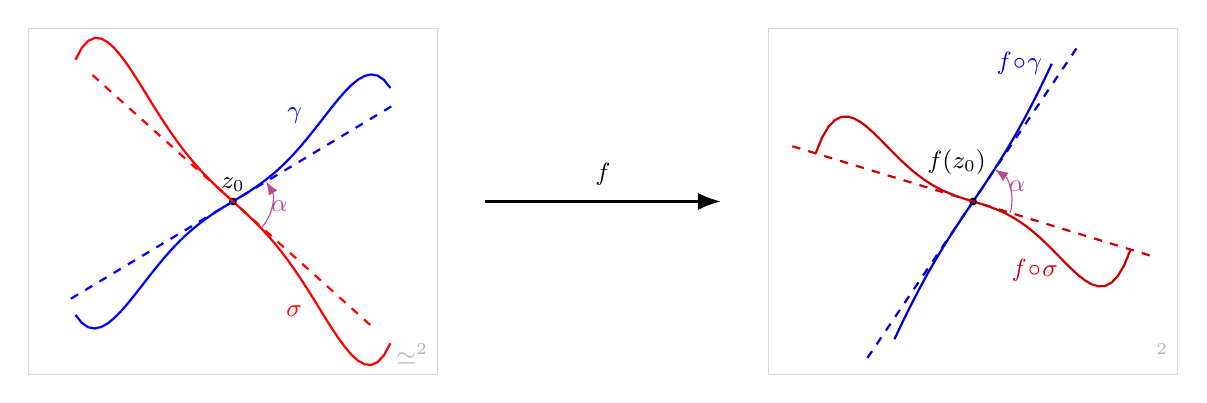
\begin{tikzpicture}[
    scale=1.0,
    >=Latex,
    every node/.style={font=\small},
]
\usetikzlibrary{arrows.meta,angles,quotes}

% ====== Parámetros ======
\pgfmathsetmacro{\mone}{0.6}    % pendiente de gamma en z0
\pgfmathsetmacro{\mtwo}{-0.9}   % pendiente de sigma en z0
\pgfmathsetmacro{\cA}{0.35}     % curvatura cúbica gamma
\pgfmathsetmacro{\cB}{0.40}     % curvatura cúbica sigma
\pgfmathsetmacro{\dA}{-0.08}    % curvatura quíntica gamma
\pgfmathsetmacro{\dB}{0.10}     % curvatura quíntica sigma

% Rotación local (diferencial de f)
\pgfmathsetmacro{\phi}{25}      

% Ángulos
\pgfmathsetmacro{\thone}{atan(\mone)}
\pgfmathsetmacro{\thtwo}{atan(\mtwo)}
\pgfmathsetmacro{\thonep}{\thone + \phi}
\pgfmathsetmacro{\thtwop}{\thtwo + \phi}

% Pendientes rotadas
\pgfmathsetmacro{\monep}{tan(\thonep)}
\pgfmathsetmacro{\mtwop}{tan(\thtwop)}
\pgfmathsetmacro{\cAp}{0.35}
\pgfmathsetmacro{\cBp}{0.40}
\pgfmathsetmacro{\dAp}{-0.08}
\pgfmathsetmacro{\dBp}{0.10}

% Largo tangentes
\pgfmathsetmacro{\L}{2.4}

% ====== Panel izquierdo ======
\begin{scope}[shift={(-4.7,0)}]
  \draw[gray!30] (-2.6,-2.2) rectangle (2.6,2.2);
  \node[anchor=south east,gray!60] at (2.6,-2.2) {$\C \simeq \R^2$};

  \coordinate (Z0) at (0,0);

  % Curva gamma con x^3 y x^5
  \draw[thick,blue,domain=-2:2,samples=50]
    plot (\x, {\mone*\x + \cA*\x^3 + \dA*\x^5});
  \node[blue,above left] at (1,{\mone*1 + \cA*1 + \dA*1}) {$\gamma$};

  % Curva sigma con x^3 y x^5
  \draw[thick,red,domain=-2:2,samples=50]
    plot (\x, {\mtwo*\x - \cB*\x^3 + \dB*\x^5});
  \node[red,below left] at (1,{\mtwo*1 - \cB*1 + \dB*1}) {$\sigma$};

  % Punto z0
  \fill (Z0) circle (1.4pt) node[above] {$z_0$};

  % Tangentes verdaderas
  \draw[dashed,blue,thick]
    ({-\L*cos(\thone)},{-\L*sin(\thone)}) -- ({\L*cos(\thone)},{\L*sin(\thone)});
  \draw[dashed,red,thick]
    ({-\L*cos(\thtwo)},{-\L*sin(\thtwo)}) -- ({\L*cos(\thtwo)},{\L*sin(\thtwo)});

  % Ángulo alpha
  \coordinate (Tg) at ({cos(\thone)},{sin(\thone)});
  \coordinate (Ts) at ({cos(\thtwo)},{sin(\thtwo)});
  \pic[draw,->,blue!40!red!70,angle radius=14pt,"$\alpha$",angle eccentricity=1.2]
      {angle = Ts--Z0--Tg};
\end{scope}

% Flecha
\draw[very thick,->] (-1.5,0) -- (1.5,0) node[midway,above=2pt] {$f$};

% ====== Panel derecho ======
\begin{scope}[shift={(4.7,0)}]
  \draw[gray!30] (-2.6,-2.2) rectangle (2.6,2.2);
  \node[anchor=south east,gray!60] at (2.6,-2.2) {$\R^2$};

  \coordinate (W0) at (0,0);

  % Imagen gamma con curvatura
  \draw[thick,blue!80!black,domain=-1:1,samples=50]
    plot (\x, {\monep*\x + \cAp*\x^3 + \dAp*\x^5});
  \node[blue!80!black,left] at (1,{\monep*1 + \cAp*1 + \dAp*1}) {$f\!\circ\!\gamma$};

  % Imagen sigma con curvatura
  \draw[thick,red!80!black,domain=-2:2,samples=50]
    plot (\x, {\mtwop*\x - \cBp*\x^3 + \dBp*\x^5});
  \node[red!80!black,below left] at (1.2,{\mtwop*1 - \cBp*1 + \dBp*1}) {$f\!\circ\!\sigma$};

  % Punto f(z0)
  \fill (W0) circle (1.4pt) node[above, yshift=6pt, xshift=-6pt] {$f(z_0)$};

  % Tangentes
  \draw[dashed,blue!80!black,thick]
    ({-\L*cos(\thonep)},{-\L*sin(\thonep)}) -- ({\L*cos(\thonep)},{\L*sin(\thonep)});
  \draw[dashed,red!80!black,thick]
    ({-\L*cos(\thtwop)},{-\L*sin(\thtwop)}) -- ({\L*cos(\thtwop)},{\L*sin(\thtwop)});

  % Ángulo alpha
  \coordinate (Tgp) at ({cos(\thonep)},{sin(\thonep)});
  \coordinate (Tsp) at ({cos(\thtwop)},{sin(\thtwop)});
  \pic[draw,->,blue!40!red!70,angle radius=14pt,"$\alpha$",angle eccentricity=1.2]
      {angle = Tsp--W0--Tgp};
\end{scope}
\end{tikzpicture}
\end{figure}
